% !TeX spellcheck = pt_PT
\documentclass[a4paper]{report}
\usepackage[portuguese]{babel}
\usepackage{a4wide}

\usepackage{graphicx}
\usepackage{hyperref}
\usepackage{listings}
\usepackage{indentfirst}
\usepackage{float}

\setlength{\parskip}{1em}

\title{POO - Trabalho Prático\\
	\large Grupo 33}
\author{Sofia Santos (A89615)
	\and Ana Filipa Pereira (A89589)
	\and Carolina Santejo (A89500)}
\date{Ano Letivo 2019/2020}

\begin{document}
	\begin{minipage}{0.9\linewidth}
        \centering
		
\includegraphics[width=0.4\textwidth]{eng.jpeg}\par\vspace{1cm}
		\href{https://www.uminho.pt/PT}
		{\scshape\LARGE Universidade do Minho} \par
		\vspace{0.6cm}
		\href{https://miei.di.uminho.pt/}
		{\scshape\Large Mestrado Integrado em Engenharia Informática} \par
		\maketitle
		\begin{figure}[H]
			
\includegraphics[width=0.32\linewidth]{sofia.jpg}
			
\includegraphics[width=0.32\linewidth]{filipa.jpg}
			
\includegraphics[width=0.32\linewidth]{santejo.jpg}
		\end{figure}
	\end{minipage}
	
	\tableofcontents
	
	\pagebreak
	
	\chapter{Introdução e principais desafios}
%	
	Este projeto consistiu no desenvolvimento de um Sistema de Gestão de Vendas (SGV) na linguagem de programação Java, sendo a continuação de um projeto anterior realizado em C. Tal como o projeto desenvolvido previamente, este é um projeto de programação em larga escala, e como foi necessário recorrer a princípios mais avançados de programação, como o uso de estruturas de dados eficientes para armazenar e consultar grandes quantidades de informação, garantindo sempre o encapsulamento dos dados. Para este projeto usámos apenas estruturas de bibliotecas standard do Java, como TreeSet ou HashMap.
	
	Neste projeto, em comparação ao anterior, foi mais fácil desenvolver formas eficazes de armazenar os dados, visto que esta linguagem de programação já nos disponibiliza bastantes estruturas de dados com vantagens diferentes, e não temos que nos preocupar com a alocação e libertação manual de memória. Para mostrar grandes quantidades de informação ao utilizador usámos o método que usámos no projeto em C, percorremos uma lista por páginas, sendo que o tamanho de cada página depende do tamanho de cada elemento, para termos algo mais consistente.
	
	\chapter{Classes, interfaces e estruturas de dados}
	\section{Catálogo (Catalog)}
	Como os catálogos de clientes e de produtos são muito parecidos, apenas muda o tipo de dados que armazenam, criámos uma interface Catalog que as classes dos catálogos de clientes e produtos implementam. Desta forma podemos dizer às classes que implementam esta interface que métodos devem implementar.
	
	\section{Clients}
	Para armazenar a informação de todos os clientes criámos a classe Clients que utiliza um TreeSet para armazenar instâncias da classe Client. A API desta classe permite realizar operações de inserção e procura.
	
	\section{Products}
	Tal como a classe dos clientes, a classe Products usa um TreeSet para armazenar instâncias da classe Product. Esta classe permite realizar operações de inserção e procura.
	
	\section{CatalogItem}
	Como usámos a interface Catalog, precisamos também de uma interface CatalogItem que as classes Client e Product implementam.
	
	\section{Client}
	Esta classe armazena informação relativa a um cliente, que no caso do nosso projeto se resume ao seu código, mas que num projeto de mais larga escala podia ser usada para armazenar outro tipo de dados, como o nome do cliente, idade, etc. A API desta classe permite validar um código de cliente e obter o código de cliente de uma instância.
	
	\section{Product}
	Tal como a classe Client, esta classe, para além de ter uma API semelhante, também armazena informação relativa a um produto, que mais uma vez inclui apenas o código de produto, mas também poderia conter mais informação, caso tal fosse relevante ou necessário.

	\section{Faturas (Bills) e Fatura (Bill)}
	Para armazenar as faturas usámos um HashMap, que associa um código de produto a uma classe à qual chamámos Bill (Fatura). Uma fatura permite armazenar, para um dado produto, o seu código, o lucro total obtido com a venda desse produto, o número total de vezes que esse produto foi vendido (registos de venda) e a quantidade total vendida. O lucro total, a quantidade total de vendas e a quantidade total vendida de um produto estão separadas por filial, mês e modo (isto é, se o produto foi comprado em promoção ou não). Temos assim a nossa definição de uma fatura:
	\begin{lstlisting}[language=Java]
public class Bill {
    private String productID;
    private double[][][] totalProfit;
    private int[][][] totalSales;
    private int[][][] totalQuantitySold;
}
	\end{lstlisting}
	A API da classe Bill permite obter informação relativa a essa fatura, e da classe Bills permite inserir faturas e obter dados relativos a todas as faturas.

	\section{Filial (Branch)}
	Para armazenar as relações entre clientes e produtos por filial usámos uma estrutura de dados constituída por dois HashMaps, um que faz corresponder cada cliente aos produtos que este comprou, e outro que faz corresponder cada produto aos clientes que o compraram. Na classe GestVendas é usada uma lista de três elementos, onde cada elemento é uma instância desta classe, para podermos ter uma instância por cada filial.\\
	\indent
	O primeiro Map (clientsWhoBought) associa cada produto (chave) aos clientes que o compraram (valor). Esta lista de clientes é outro HashMap, que a cada cliente (chave) faz corresponder a informação relativa à compra do produto inicial por esse cliente (valor), nomeadamente a quantidade desse produto comprada, o número de registos de venda e o dinheiro gasto nesse produto, todos divididos por mês.\\
	\indent
	O segundo Map (productsBoughtBy) associa cada cliente (chave) aos produtos que este comprou (valor). Tal como no outro Map, neste a lista de produtos é também um HashMap, que a cada produto (chave) faz corresponder a informação relativa à compra desse produto pelo cliente inicial (valor). Esta informação inclui a quantidade desse produto comprada, o dinheiro gasto nesse produto e o número de registos de venda associados ao cliente dado, todos divididos por mês.\\
	\indent
	A informação dos clientes e dos produtos mencionada acima é armazenada em instâncias da classe CliProdInfo.
	\indent
	Estes dois HashMaps acabam por conter na sua maioria a mesma informação, mas esta duplicação de informação resulta numa enorme eficiência na execução das queries. Se apenas tivéssemos o Map que associa cada produto aos clientes que o compraram, por exemplo, e quiséssemos uma lista de todos os produtos comprados por um dado cliente, teríamos que percorrer o Map todo, visto que o cliente pode ter comprado qualquer produto, enquanto que usando dois Maps podemos simplesmente consultar uma vez o HashMap que associa cada cliente aos produtos que comprou e teríamos imediatamente a nossa resposta. Passamos assim de milhares de consultas a poucas dezenas (a complexidade passa de O(N) para O(log N), e como temos milhares de clientes e de produtos, a diferença é significativa).\\
	\indent
	Esta classe permite realizar operações de inserção, pesquisa e obtenção de dados.
	
	\section{Informação dos ficheiros (FileInfo)}
	Esta classe armazena informação relativa aos ficheiros lidos aquando do carregamento do GestVendas, nomeadamente os caminhos dos ficheiros, o número total de linhas e o número de linhas válidas. Em relação às vendas, são guardados também a faturação total, o número de vendas de custo 0 e o número de clientes que fizeram compras, para responder à primeira consulta estatística. Esta classe permite realizar operações de consulta e alteração de dados.
	
	\section{StructuresInfo}
	Esta classe armazena a informação necessária para responder à segunda consulta estatística, mais nomeadamente o número total de compras por mês, a faturação total por mês e filial, tal como o valor global, e o número de distintos clientes por mês e por filial.

	\section{GestVendas}
	O nosso Sistema de Gestão de Vendas é composto pelas seis estruturas principais mencionadas acima. A classe GestVendas permite preencher as suas variáveis de instância a partir de ficheiros e responde a todas as queries.
	Podemos então definir a nossa classe GestVendas da seguinte forma:
	\begin{lstlisting}[language=Java]
public class GestVendas {
    private Clients clients;
    private Products products;
    private Bills bills;
    private ArrayList<Branch> branches;
    private FileInfo fileInfo;
    private StructuresInfo structuresInfo;
}
	\end{lstlisting}
	Esta classe também permite que armazenemos o seu estado atual através de ObjectStreams, e permite carregar um estado armazenado em disco.
	
	\section{Venda (Sale)}
	Definimos uma classe auxiliar que nos permite armazenar uma venda, tal como consta no ficheiro das vendas. Esta classe permite-nos aceder à informação de cada venda de forma mais eficiente, aquando do preenchimento dos módulos das faturas e das filiais. Esta classe apenas inclui operações de criação, consulta de dados e validação de uma venda, visto que é uma classe temporária, que apenas é usada para auxiliar o carregamento de dados dos ficheiros na GestVendas.
		
	\section{UI/QueriesUI}
	As classe UI e QueriesUI, tal como os nomes indicam, tratam da parte visual do programa, como mostrar ao utilizador os resultados das queries, os menus do programa, e os \textit{input prompts}. Através da classe Formatting, foi possivel imprimir texto colorido no terminal. A classe UI trata da User Interface geral do programa, enquanto que a classe QueriesUI é específica das queries, tornando assim o código mais organizado.
	
	\section{Queries}
	A classe Queries é a responsável pelo fluxo das queries, ou seja, é a que trata de receber \textit{input} do utilizador, chamar a função da query correspondente, fornecendo-lhe o \textit{input} necessário, e enviar o \textit{output} para a classe QueriesUI, para poder ser apresentado ao utilizador.
	
	\section{Controlador (Controller)}
	Por último, a classe Controlador é a classe principal, ou seja, é esta que controla o fluxo de todo o programa. Esta classe controla que query será executada, ou que ficheiros serão carregados no programa. A classe GestVendasAppMVC, a que contém o método main, é apenas responsável por correr o método run da classe Controller, a partir daí o Controller trata de correr o programa.
	
	\chapter{Estrutura do projeto}
	
	O nosso projeto segue a estrutura \textit{Model View Controller} (MVC), estando por isso organizado em três camadas:
	\begin{itemize}
		\item A camada de dados (o modelo) é composta pela classe GestVendas, que por sua vez é constituído pelas classes referidas no capítulo anterior, Clients, Products, Bills, Branch, FileInfo e StructuresInfo. Para além destas, temos ainda a classe auxiliar Venda, e as subclasses Client, Product e Bill.
		\item A camada de interação com o utilizador (a vista, ou apresentação) é composta pelas classes UI e QueriesUI.
		\item A camada de controlo do fluxo do programa (o controlador) é composta pelas classes Controller e Queries. É esta camada que gere o funcionamento do programa, interagindo com as outras duas camadas para que este possa funcionar da forma pretendida. As outras duas camadas nunca interagem diretamente uma com a outra.
	\end{itemize}
	Nesta estrutura, o controlador é responsável por enviar pedidos ao modelo, como por exemplo responder a uma query. O modelo calcula essa resposta e envia-a ao controlador, que irá pedir à vista para a apresentar ao utilizador. Temos assim três camadas distintas que funcionam juntas para formar o nosso programa.

	\chapter{Complexidade das estruturas}
	
	Decidimos usar TreeSets nos catálogos de clientes e de produtos para podermos aceder aos dados dos catálogos de forma ordenada. Podíamos ter usado HashSets, por exemplo, mas nesse caso teríamos que ordenar os dados sempre que fôssemos aceder a instâncias dessas classes, o que iria ter um grande impacto na performance, e implicaria mudar a primeira query para passar a ordenar a lista que devolve.
	
	Para os dados das faturas, usámos HashMaps em vez de TreeMaps puramente por escolha nossa. Comparando os tempos médios de execução das queries 5 a 9, em segundos, usando ambas as estruturas vemos que a diferença é tão pequena que não terá um impacto significante no desempenho do nosso programa, e podemos assim usar qualquer uma das duas estruturas.
	\begin{center}
		\begin{tabular}[pos]{| c | c | c |}
			\hline
			Query & HashMap & TreeMap \\ \hline
			5 & 0.0022 & 0.0020 \\ \hline
			6 & 0.6347 & 0.6733 \\ \hline
			7 & 0.4939 & 0.4849 \\ \hline
			8 & 0.3838 & 0.3511 \\ \hline
			9 & 0.0003 & 0.0004 \\ \hline
		\end{tabular}
	\end{center}
	
	Para os dados das filiais usámos HashMaps porque a performance com HashMaps é melhor, em geral, em comparação com TreeMaps, apesar da diferença não ser muito significativa. A única query que sofre bastante com esta troca é a query 10, cujo tempo de execução quase que duplica. Nesta tabela é possível ver o tempo médio de execução das queries 5 a 9 usando HashMaps e TreeMaps, em segundos (o ficheiro de vendas usado é o de 1 milhão de vendas):\\
	\begin{center}
	\begin{tabular}[pos]{| c | c | c |}
		\hline
		Query & HashMap & TreeMap \\ \hline
		5 & 0.0022 & 0.0015 \\ \hline
		6 & 0.6347 & 0.6509 \\ \hline
		7 & 0.4939 & 0.6376 \\ \hline
		8 & 0.3838 & 0.4450 \\ \hline
		9 & 0.0003 & 0.0003 \\ \hline
	\end{tabular}
	\end{center}
	
	No caso das estruturas relativas aos resultados das queries, foi utilizada a mais adequada para cada situação, como Maps ou Lists.

	\chapter{Testes de desempenho}
	
	Para medir o desempenho do programa usámos duas classes, a classe Benchmark para medir o tempo médio de execução das queries, e a classe PerformanceTests, para medir o tempo de leitura dos ficheiros de vendas, com ou sem parsing e validação. Estas classes podem ser corridas em separado do resto do programa, permitindo-nos realizar estes testes sem interferir com o programa principal. Estas classes usam a classe Crono para medir os tempos de execução.
	
	A seguinte tabela permite-nos visualizar os tempos médios de execução de cada query, em segundos, para cada um dos três ficheiros de vendas (o tempo médio é a média do tempo de execução de 5 medições):
	\begin{center}
	\begin{tabular}[pos]{| c | c | c | c |}
		\hline
		Query & 1M Vendas & 3M Vendas & 5M Vendas \\ \hline
		1 & 0.0437 & 0.0559 & 0.0471\\ \hline
		2 & 0.4937 & 1.0281 & 1.1121\\ \hline
		3 & 0.0023 & 0.0006 & 0.0044\\ \hline
		4 & 0.0010 & 0.0003 & 0.0013\\ \hline
		5 & 0.0022 & 0.0010 & 0.0027\\ \hline
		6 & 0.6347 & 0.9005 & 0.9428\\ \hline
		7 & 0.4939 & 1.5213 & 1.6373\\ \hline
		8 & 0.3838 & 1.9895 & 3.8710\\ \hline
		9 & 0.0003 & 0.0001 & 0.0005\\ \hline
		10 & 2.6814 & 12.523 & 23.925\\ \hline
	\end{tabular}
	\end{center}

	Pela análise da tabela, podemos concluir o seguinte:
	\begin{itemize}

		\item para a maioria das queries, o tempo de execução não sofre uma alteração muito grande com o aumento do número de vendas.

		\item as queries cujo tempo de execução é afetado pela quantidade de vendas são as queries 2, 6, 7, 8 e 10, com a query 10 sendo a mais afetada.
		
	\end{itemize}

	Para além dos testes de tempo de execução, realizámos também testes de performance da leitura dos ficheiros de vendas, cujos resultados podem ser consultados na seguinte tabela:
	\begin{center}
	\begin{tabular}[pos]{| c | c | c | c |}
		\hline
		Tipo de teste & 1M Vendas & 3M Vendas & 5M Vendas \\ \hline
		Leitura & 0.5403 & 1.2304 & 2.0249\\ \hline
		Leitura + parsing & 2.2272 & 6.1081 & 10.028\\ \hline
		Leitura + parsing + validação & 3.1269 & 9.1028 & 16.245\\ \hline
	\end{tabular}
	\end{center}
	Esta tabela mostra-nos aquilo que já seria de esperar. Quantas mais vendas contiver o ficheiro que estamos a ler, maiores vão ser os tempos de leitura, parsing e validação. Vemos também que o que mais afeta o tempo de execução é o parsing de cada linha, mais do que a validação e mais do que o número de vendas.

	\chapter{Conclusão}

	Tal como o projeto em C, sentimos que o nosso projeto está bem conseguido. O nosso programa é capaz de responder a todas as queries e mostrar os resultados de forma intuitiva, e fá-lo com tempos aceitáveis.
	
	Tentámos melhorar a estrutura do projeto quando passámos de C para Java, o que tínhamos feito em C estava um pouco confuso e complexo, e acreditamos que neste projeto conseguimos simplificar algumas coisas, tornando o código mais simples de ser entendido por alguém que o veja.
	
	\appendix
	
	\chapter{Diagrama de Classes}
	\begin{figure}[H]
		\begin{center}
			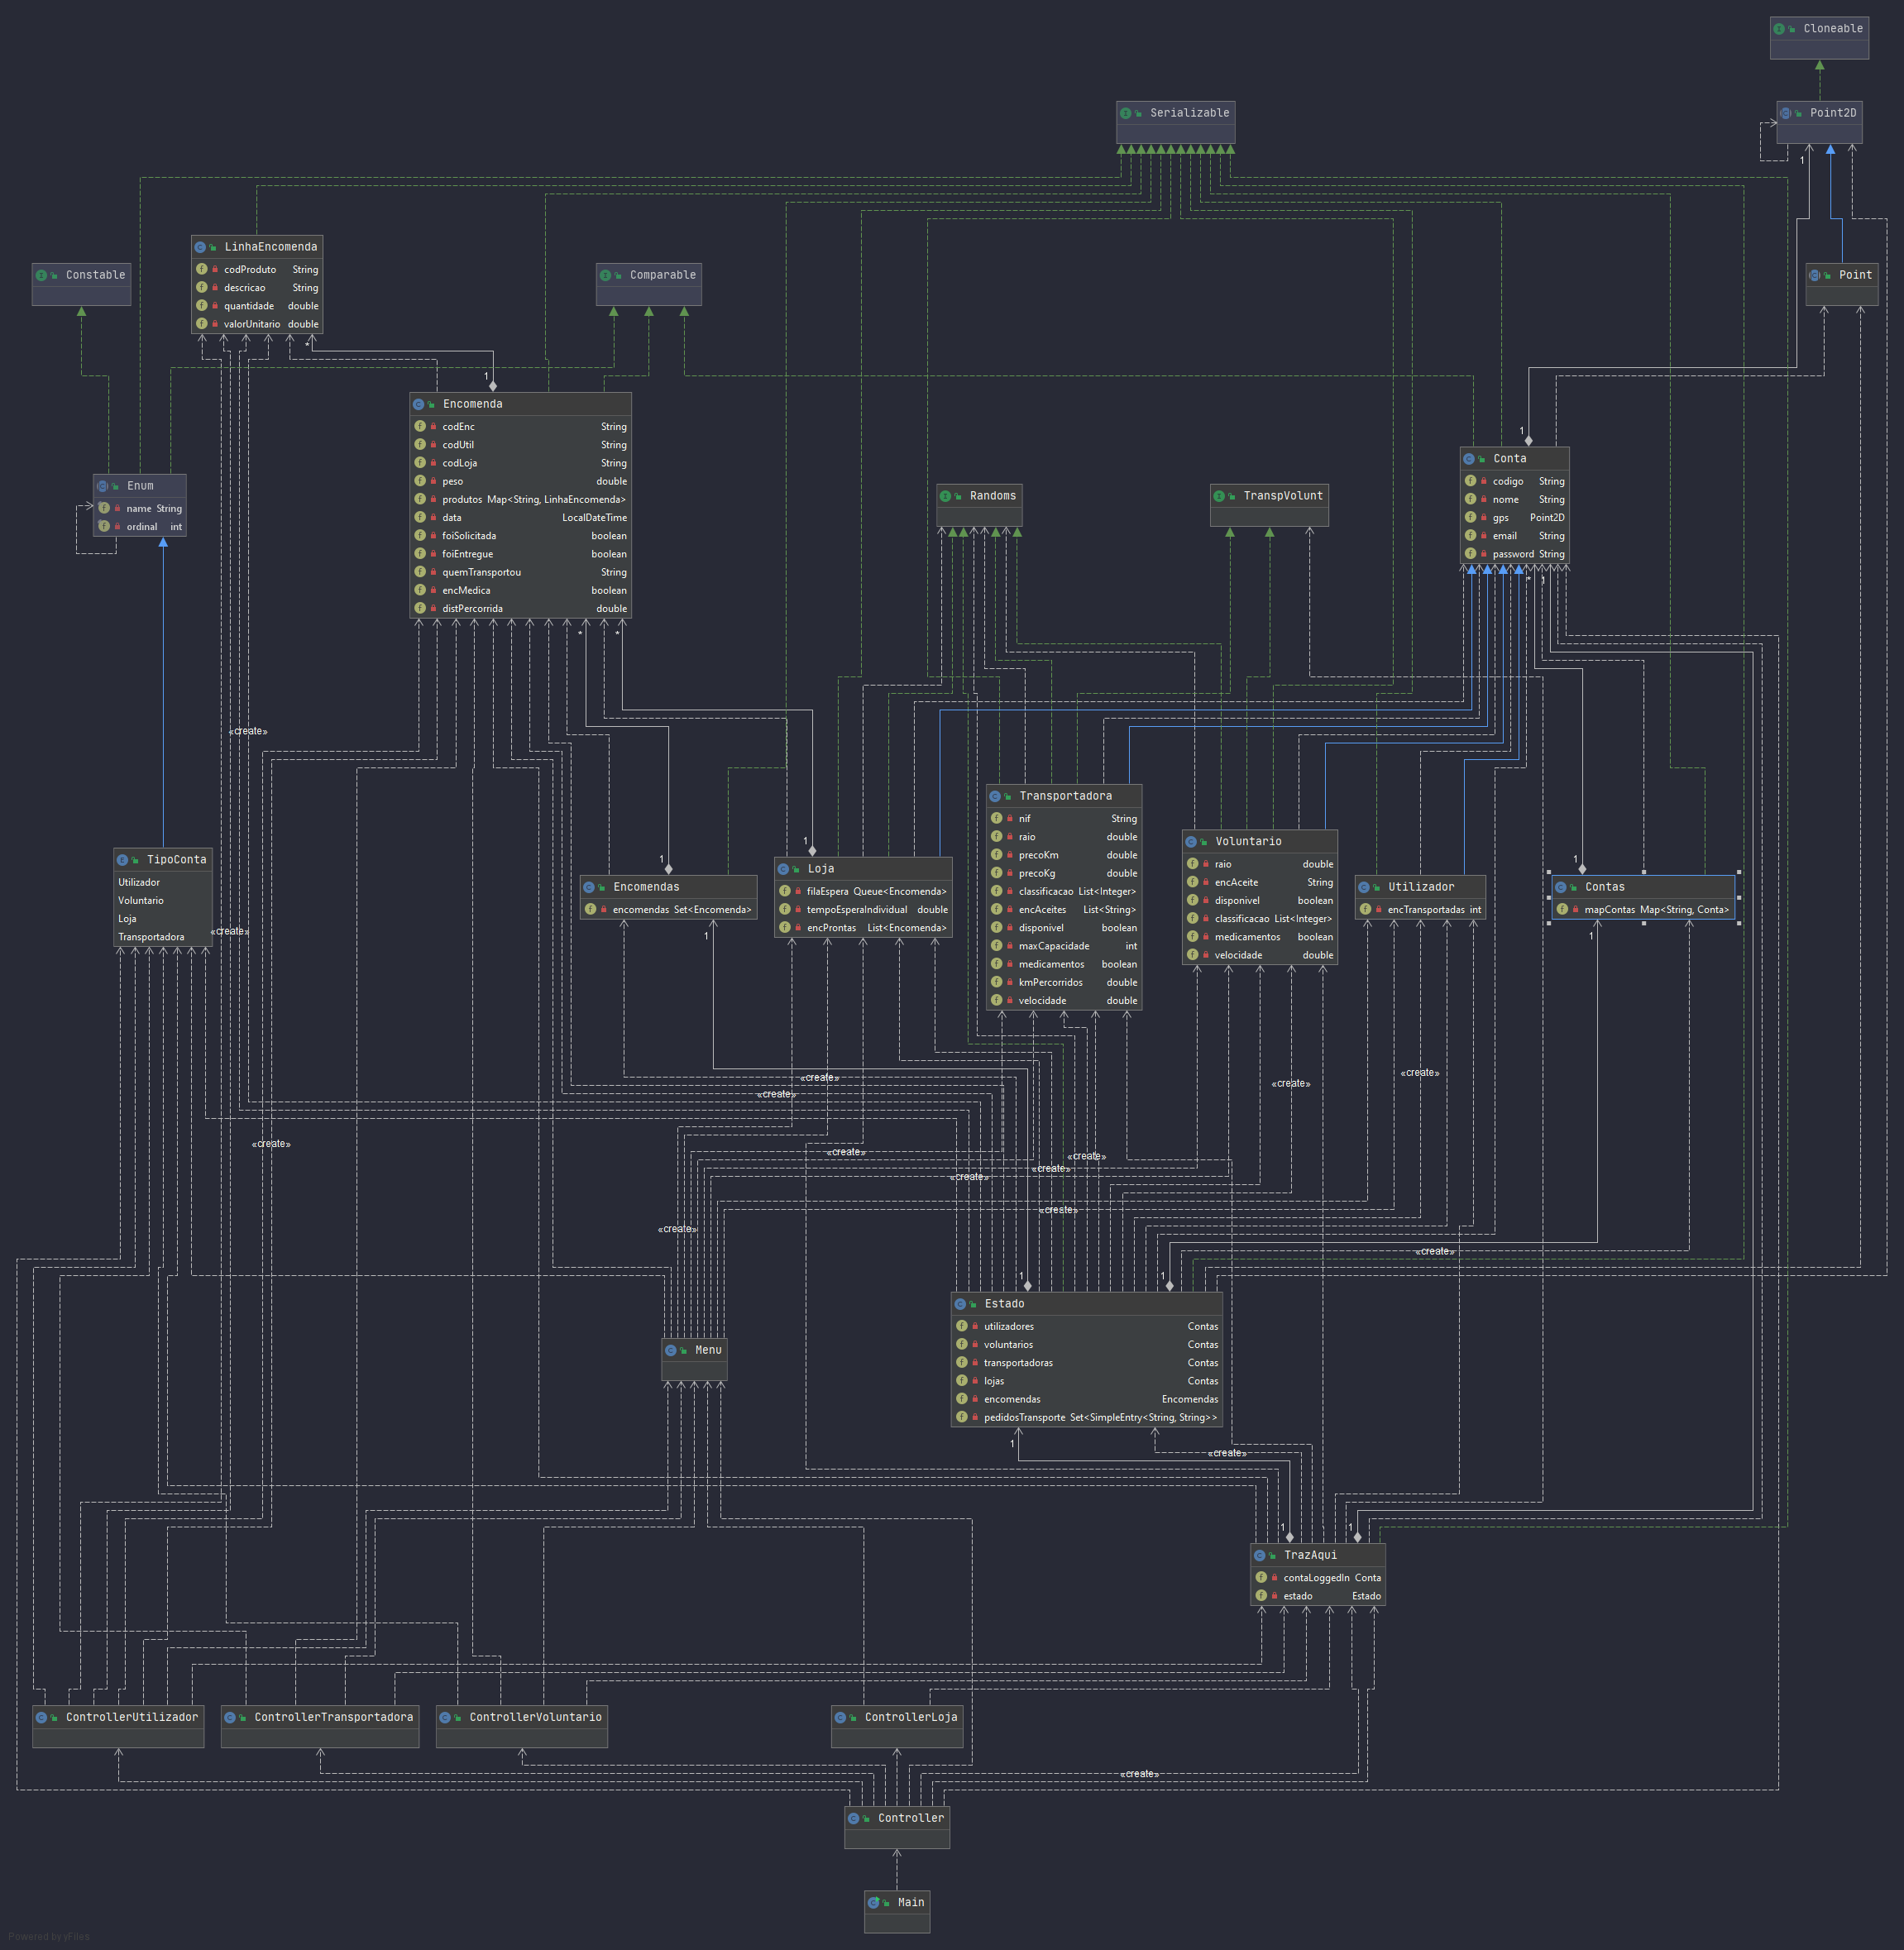
\includegraphics[height=0.6\textheight]{DiagramaDeClasses.png}
			\caption{Diagrama de classes do programa, gerado pelo \emph{IntelliJ}}
		\end{center}
	\end{figure}
\end{document}